\documentclass[../sparc.tex]{subfiles}
\graphicspath{{\subfix{../images/}}}
\begin{document}

%%%%%%%%%%%%%%%%%%%%%%%%%%%%%%%%%%%%%%%%%%%%%%%%%%%%%%%%%%%%%%%%%%%%%%%%%%%%%%%%
\section{Half-tones, sharps and flats}

All this chapter we were saying that there are eight notes in the octave and we
have 63 different sounds (notes) in all octaves in total.  But in fact that's
not accurate -- it turns out that there twelve sounds in the octave instead of
eight!

What a surprise!  How we get those five sounds in additional to the eight basic
ones?  We get those sounds because we have so called \emph{half-tones} in music,
that allow us to spice up our music with additional sounds.

The most convenient way to see those half-tones is to look on a piano keyboard,
part of which is shown on fig. \ref{fig:piano-keyboard}.

\begin{figure}[ht]
  \centering
  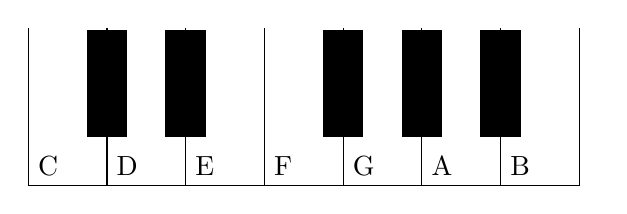
\begin{tikzpicture}
    \draw (0, 0) -- (7, 0);
    \foreach \x/\note in {0/C, 1/D, 2/E, 3/F, 4/G, 5/A, 6/B, 7/} {
      \draw (\x, 0) -- (\x, 2) -- (\x, 0) node[anchor=south west] {\note};
    };
    \foreach \x in {1, 2, 4, 5, 6} {
      \node[
        rectangle,
        draw,
        fill=black,
        minimum width=0.5cm,
        minimum height=1.35cm
      ] (r) at (\x, 1.30) {};
    };
  \end{tikzpicture}
  \label{fig:piano-keyboard}
  \caption{One octave on a piano keyboard.}
\end{figure}

We can see from this figure that between some pair of notes, namely ``C''--``D'',
``D''--``E'', ``F''--``G'', ``G''--``A'', ``A''--``B'' there are additional black
keys.  If we count all the keys on one octave, we will get 12 keys -- or 12
sounds.

That can be explained by the fact that the distance between two adjacent keys in
the frequency range on a piano keyboard is \emph{one half-tone}.  Most of the
white keys have enough space between them in terms of the frequencies to squeeze
one additional key between them (two pairs ``B''--``C'' and ``E''--``F'' are the
exceptions.)

There are no special ``squiggles'' for marking such sounds in the music, but we
have special ``modifiers'' for the main seven notes, that makes the frequency of
the note one half-tone higher or lower.

For example, to get the frequency of the black key between the pair ``C''--``D'',
we can raise the frequency of ``C'' by a half-tone, of lower the frequency of
``D'' half-tone down.

The modifier that makes the frequency of a note half-tone higher is called
\emph{sharp}, and the similar modifier that makes the frequency half-tone lower
is called \emph{flat}.

\index{Музыка!Диез}

The notes with the ``sharp'' modifier are marked with ``\#'' symbol that goes
before the note -- as is shown on the fig. \ref{fig:lilypond-f4-sharp}.

\begin{figure}[ht]
  \centering
  \begin{lilypond}
    \relative c' {
      \numericTimeSignature
      \time 4/4
      fis4
    }
  \end{lilypond}
  \caption{``F Sharp'' from the 4th octave.}
  \label{fig:lilypond-f4-sharp}
\end{figure}

We can easily calculate the frequency of ``F4\#'' using the frequencies of
``F4'' and ``G4''.  Note that we named the constant as \texttt{f4s}, using ``s''
as the shorthand for ``sharp'', because we cannot use ``\#'' in variable and
constant names.

\begin{listing}[ht]
  \begin{minted}{cpp}
    const float f4  = 349.230;
    const float g4  = 392.000;
    const float f4s = (f4 + g4) / 2; // F4 Sharp
  \end{minted}
  \label{listing:music-f4-sharp}
  \caption{Calculation of the sharp of a note.}
\end{listing}

This approach works for other notes as well.

By the way, for those notes that do not have a black key after them (``B'',
``E''), the sharp is just the next regular note.  For example, ``E4\#'' is
``F4'' and ``B4\#'' is no more than ``C5''.

Thus:

\begin{listing}[ht]
  \begin{minted}{cpp}
    const float e4  = 329.630;
    const float f4  = 349.230;
    const float e4s = f4; // E4 Sharp
  \end{minted}
  \caption{The distance between some main notes is exactly half-tone.}
  \label{listing:music-e4-sharp}
\end{listing}

\index{Музыка!Бемоль}

Flats works with the same logic as the sharps, except they \textbf{lower} the
note by a half-tone.  They are marked with the special symbol ``\flat'' before the
note that is under this ``flat'' modifier.

Let's take ``E4\flat'' as an example (as is shown on
fig. \ref{fig:lilypond-e4-flat}.)

\begin{figure}[ht]
  \centering
  \begin{lilypond}
    \relative c' {
      \numericTimeSignature
      \time 4/4
      ees4
    }
  \end{lilypond}
  \caption{``E Flat'' of the 4th octave.}
  \label{fig:lilypond-e4-flat}
\end{figure}

The flat of ``E4'' is the frequency between ``E4'' and the previous note, which
is ``D4'' -- as is shown in the formula \ref{equation:e-flat-calculation}.

\begin{equation}
  \frac{\mbox{E4} + \mbox{D4}}{2} = \mbox{E4\flat}
  \label{equation:e-flat-calculation}
\end{equation}

We will be using ``f'' as the marker of ``flat'' note in the programming
code.\footnote{In the music notation you sometimes can find double-sharps or
double-flats, which means that we have to raise the frequency of a note two of
half-tones up, or lower the same number of steps down.}

\begin{listing}[ht]
  \begin{minted}{cpp}
    const float d4  = 293.660;
    const float e4  = 329.630;
    const float e4f = (e4 + d4) / 2; // E4 Flat
  \end{minted}
  \label{listing:music-e4-flat}
  \caption{Calculation of a ``flat'' note.}
\end{listing}

Up till now we discussed all those sharps and flats in variants where the
modifier was written right before a note, that are under the ``influence'' of
this ``spell'' -- we call those ``ad-hoc symbols'' (or ``accidentals''.)  But it
is not very convenient for musicians to write down such modifiers before each
note, especially when there are lots of notes in a musical composition.  To
solve this problem, we use sharps and flats that are written at the beginning of
the musical staff.  The influence of such symbols is extends on all notes of the
same kind across all musical staff.

Let's get back to the ``If only there will be no winter'' composition on
fig. \ref{fig:lilypond-melody-prostokvashino}.  If we look closely on the
musical staff we should note that there'is ``\#'' symbol at the beginning, on
the line that represents ``F5'' -- which means that all ``F'' notes must be
sharps, unless otherwise noted.

\begin{tikzpicture}
  \node (image) at (4, 0) {
    \begin{lilypond}
      \relative c' {
        \key g \major
        \numericTimeSignature
        \time 4/4
        b8 b b'8. fis16 a8 g e4 |
        d8 d << b'8. d8. >> << c16 a >> << c8 a >> << b8 g8 >> r4
      }
      \layout {
        indent = 0\mm
        line-width = 120\mm
        ragged-last = ##t
      }
    \end{lilypond}
  };
  \draw[red, thick, ->] (0.0, 1.0) node[anchor=south west] {F5 Sharp}
  -- (-0.5, 0.5);
  \label{fig:lilypond-melody-prostokvashino-2}
\end{tikzpicture}

With this knowledge we can improve our programming code for the melody.

\begin{listing}[ht]
  \begin{minted}{cpp}
    const float f4s = (f4 + g4) / 2;

    // ...

    float prostokvashino[28][2] = {
      // 1st bar.
      {b3,  8},  {b3, 8}, {b4, 16.0 / 3.0},
      {f4s, 16}, {a4, 8}, {g4,          8}, {e4, 4},
      // 2nd bar.
      {d4,  8},  {d4, 8}, {d5, 16.0 / 3.0},
      {c5,  16}, {c5, 8}, {b4,          8}, {R,  4},
      // 3rd bar.
      {d5,  8},  {c5, 8}, {a4,          8},
      {f4s, 8},  {c5, 8}, {b4,          8}, {b4, 4},
      // 4th bar.
      {b3,  8},  {b3, 8}, {b4, 16.0 / 3.0},
      {a4,  16}, {a4, 8}, {g4,          8}, {R,  4},
    };

    // ...
  \end{minted}
  \label{listing:prostokvashino-with-shaprs}
  \caption{Improved version of ``If only there will be no winter'' melody with
    added sharps.}
\end{listing}

\end{document}
